\documentclass[notes, c, 11pt, xcolor=dvipsnames, hyperref={colorlinks,citecolor=Maroon,linkcolor=Maroon,urlcolor=RoyalBlue}]{beamer}

% print notes only:
%\documentclass[notes=only, c, 11pt, xcolor=svgnames, hyperref={colorlinks,citecolor=DeepPink4,linkcolor=DarkRed,urlcolor=DarkBlue}]{beamer}

% print only frames:
%\documentclass[c, 11pt, xcolor=svgnames, hyperref={colorlinks,citecolor=DeepPink4,linkcolor=DarkRed,urlcolor=DarkBlue}]{beamer}

% print handouts:
%\documentclass[handout, c, 11pt, xcolor=svgnames, hyperref={colorlinks,citecolor=DeepPink4,linkcolor=DarkRed,urlcolor=DarkBlue}]{beamer} 
%\usepackage{pgfpages}
%\pgfpagesuselayout{4 on 1}[a4paper, border shrink=5mm, landscape]

\setbeamerfont{note page}{size=\tiny}

\usepackage[english]{babel}
\usepackage[latin1]{inputenc}
\usepackage[T1]{fontenc}

\mode<presentation> {
	
	% The Beamer class comes with a number of default slide themes
	% which change the colors and layouts of slides. Below this is a list
	% of all the themes, uncomment each in turn to see what they look like.
	
	%\usetheme{default}
	%\usetheme{AnnArbor}
	%\usetheme{Antibes}
	%\usetheme{Bergen}
	%\usetheme{Berkeley}
	%\usetheme{Berlin}
	%\usetheme{Boadilla}
	\usetheme{CambridgeUS}
	%\usetheme{Copenhagen}
	%\usetheme{Darmstadt}
	%\usetheme{Dresden}
	%\usetheme{Frankfurt}
	%\usetheme{Goettingen}
	%\usetheme{Hannover}
	%\usetheme{Ilmenau}
	%\usetheme{JuanLesPins}
	%\usetheme{Luebeck}
	%\usetheme{Madrid}
	%\usetheme{Malmoe}
	%\usetheme{Marburg}
	%\usetheme{Montpellier}
	%\usetheme{PaloAlto}
	%\usetheme{Pittsburgh}
	%\usetheme{Rochester}
	%\usetheme{Singapore}
	%\usetheme{Szeged}
	%\usetheme{Warsaw}
	
	% As well as themes, the Beamer class has a number of color themes
	% for any slide theme. Uncomment each of these in turn to see how it
	% changes the colors of your current slide theme.
	
	%\usecolortheme{albatross}
	%\usecolortheme{beaver}
	%\usecolortheme{beetle}
	%\usecolortheme{crane}
	%\usecolortheme{dolphin}
	%\usecolortheme{dove}
	%\usecolortheme{fly}
	%\usecolortheme{lily}
	%\usecolortheme{orchid}
	%\usecolortheme{rose}
	%\usecolortheme{seagull}
	%\usecolortheme{seahorse}
	%\usecolortheme{whale}
	%\usecolortheme{wolverine}
	
	\usefonttheme{professionalfonts}
	
	\usepackage{times}
	\usepackage{tikz}
	\usetikzlibrary{arrows,shapes}
	
	%\setbeamertemplate{footline} % To remove the footer line in all slides uncomment this line
	%\setbeamertemplate{footline}[page number] % To replace the footer line in all slides with a simple slide count uncomment this line
	\setbeamertemplate{headline} % to remove header with navigation tree
	
	\setbeamertemplate{navigation symbols}{} % To remove the navigation symbols from the bottom of all slides uncomment this line
}

\usepackage{amsmath,mathtools}
\usetikzlibrary{matrix, fit, backgrounds}

\usepackage{graphicx} % Allows including images
\usepackage{booktabs} % Allows the use of \toprule, \midrule and \bottomrule in tables
\usepackage{subcaption}
\usepackage{tabularx}

\usepackage{fancyvrb}

\usetikzlibrary{mindmap,trees,shadows,backgrounds}

%\tikzset{every node/.append style={scale=0.6}}    

\usepackage{array,multirow}
\usepackage{changepage}

\usepackage[backend=biber, style=authoryear-comp, citestyle=authoryear-comp, firstinits=true, url=false, doi=false, eprint=false, dashed=false, maxbibnames=99]{biblatex}
\addbibresource{bib.bib}

%----------------------------------------------------------------------------------------
%	TITLE PAGE
%----------------------------------------------------------------------------------------

\title[Webinar for ISDS R Group]{Building meaningful machine learning models for disease prediction} % The short title appears at the bottom of every slide, the full title is only on the title page

\author{Dr Shirin Glander} % Your name
\institute[] % Your institution as it will appear on the bottom of every slide, may be shorthand to save space
{
	Dep. of Genetic Epidemiology \\
	Institute of Human Genetics \\
	University of M\"unster
	
	\vspace{0.5cm} 
	
	\href{mailto:shirin.glander@wwu.de}{shirin.glander@wwu.de} \\
	
	\vspace{0.5cm} 
	
	\href{https://shiring.github.io}{https://shiring.github.io} \\
	
	\href{https://github.com/ShirinG}{https://github.com/ShirinG}
	
}
\date{Friday, 31\textsuperscript{st} March 2017} 

\AtBeginSection[]{
	\begin{frame}
		\vfill
		\centering
		\begin{beamercolorbox}[sep=8pt,center,shadow=true,rounded=true]{title}
			\usebeamerfont{title}\insertsectionhead\par%
		\end{beamercolorbox}
		\vfill
	\end{frame}
}

%\renewcommand{\thefootnote}{$\star$} 

%%%%%%%%%%%%%%%%%%%%%
%	TITLE PAGE
%%%%%%%%%%%%%%%%%%%%%

\begin{document}
	
	\begin{frame}
		\titlepage
	\end{frame}
	
\note{
	\begin{itemize}
		\item Welcome everybody!
		\item Thank you very much for the invitation and the opportunity to present this talk
		\item I will go over my work on using machine learning models in disease prediction
		\item I want to specifically give a hands-on demonstration of how you can build meaningful models yourselves using R
		\item I will demonstrate how to evaluate model performance and
		\item how to optimize models to address different disease-related questions
	\end{itemize}
}

%%%%%%%%%%%%%%%%%%%%%
%	ABOUT ME
%%%%%%%%%%%%%%%%%%%%%

\begin{frame}
	\frametitle{About me}
	
	\begin{columns}
		\column{0.15\textwidth}	
	
		\column{0.8\textwidth}	
	\begin{itemize}		
		\item[since 2015] Bioinformatics Postdoc \\
							Next Generation Sequencing \\
							autoinflammatory diseases \& \\
							innate immunity \\[5mm]
		\item[2011 - 2015] PhD in Biology \\
							Is the immune system of plants required to adapt to flowering time change? \\[5mm]
		\item[2005 - 2011] BSc and MSc of Science in Biology \\
							evolutionary genetics, \\ immune memory in Drosophila \\				
	\end{itemize}

	\column{0.05\textwidth}	
	
	\begin{tikzpicture}[remember picture,overlay]
	\node[xshift=-2.1cm,yshift=-2.5cm] at (current page.north east) {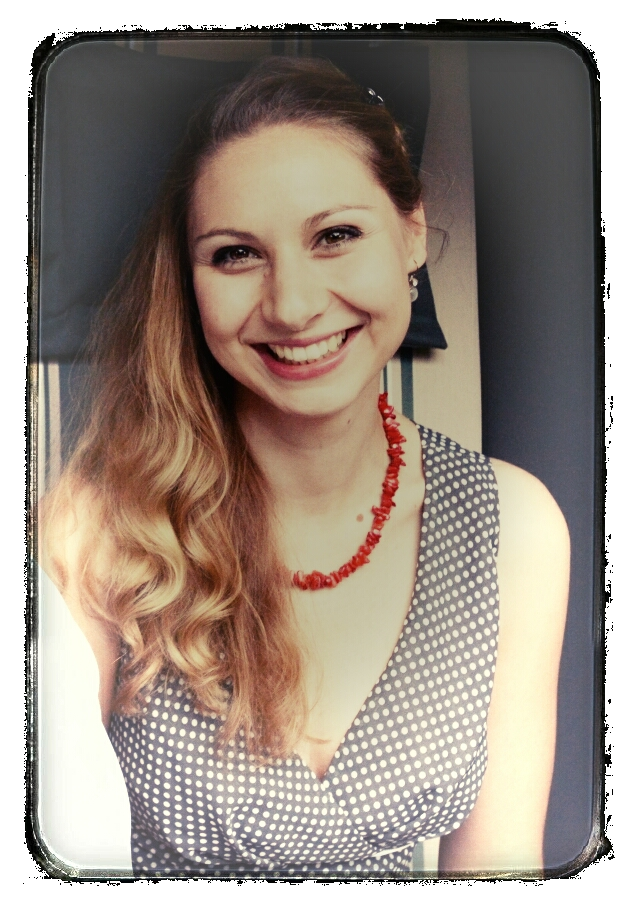
\includegraphics[width=3cm]{images/bild.png}};
	\end{tikzpicture}

	\end{columns}
\end{frame}

\note{
	\begin{itemize}
		\item Before I start, I want to quickly introduce myself:
		\item I am a bioinformatics postdoc
		\item working with next generation sequencing data,
		\item like RNA-seq for transcriptomics,
		\item whole genome sequencing for variant analysis,
		\item ATAC- or Chip-seq for chromatin and epigenetic information.
		\item My own research focuses on questions relating to autoinflammatory diseases
		\item and innate immune mechanisms
	\end{itemize}
	
	\begin{itemize}
		\item I earned my PhD in biology from the University of M�nster in 2015
		\item working with RNA-seq data to determine how plant defense has co-evolved with and potentially shaped different life-history strategies
	\end{itemize}
	
	\begin{itemize}
		\item Before that, during my BSc and MSc I worked on questions about evolutionary genetics and immune memory in Drosophila
		\end{itemize}
}

%%%%%%%%%%%%%%%%%%%%%
%	TABLE OF CONTENTS
%%%%%%%%%%%%%%%%%%%%%

	\begin{frame}[c]
		\frametitle{Table of contents}
		\alert{Building meaningful machine learning models for disease prediction}
		\vspace{0.5cm}
			\tableofcontents[hideallsubsections]

	\end{frame}

\note{
	\begin{itemize}
		\item Now, let's start with the topic about which you're here:
		\item Machine learning is a powerful approach for developing sophisticated, \\
			automatic, and objective models for the analysis of complex biomedical data
		\item Machine learning promises to help physicians make near-perfect diagnoses, ...
		\item ... choose the best medications for their patients, ...
		\item ... predict readmissions, ...
		\item ... identify patients at high-risk for poor outcomes, ...
		\item ... and in general improve patients' health while minimizing costs. 
	\end{itemize}
	
	\begin{itemize}
		\item I titled my talk: "Building meaningful machine learning models for disease prediction"
		\item with the emphasis on \textbf{meaningful}
		\item So, first, I want to introduce to you what it is I mean exactly with \textbf{meaningful models}
		\item Then, I will give you a few examples of how machine learning is currently being used in disease modeling and clinical data science
		\item Before I delve into the nitty-gritty of modeling, I will quickly recap the most important concepts of ML
		\item And finally, I will show how to build ML models in R
		\item and how to evaluate the performance of such models
	\end{itemize}
}

%%%%%%%%%%%%%%%%%%%%%
%	SECTION
%	What makes a model meaningful?
%%%%%%%%%%%%%%%%%%%%%

\section{What makes a model meaningful?}

\begin{frame}
	\frametitle{What makes a model meaningful?}
	
	\alert{\textsl{Meaningful} models}
	\vspace{0.2cm}
	
	\begin{itemize}
		\item answer the question(s) posed...
		\item ... with sufficient accuracy to be trustworthy
		\item are generalizable
	\end{itemize}

	\vspace{0.6cm}

	\begin{center}
		{\Large \alert{Accuracy depends on the problem!}}
		
		\vspace{1cm}
		
		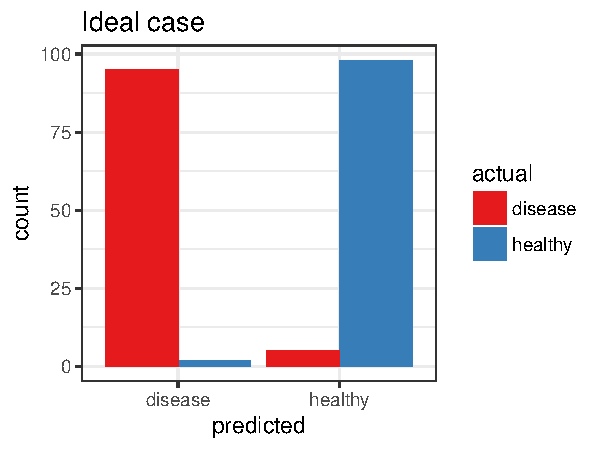
\includegraphics[width=0.33\textwidth]{images/meaningful_1}
		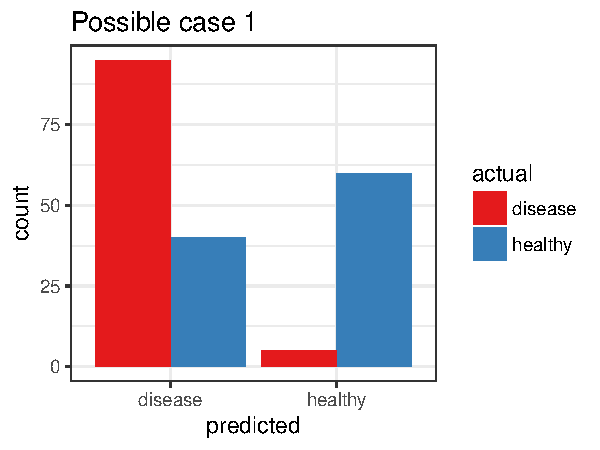
\includegraphics[width=0.33\textwidth]{images/meaningful_2}
		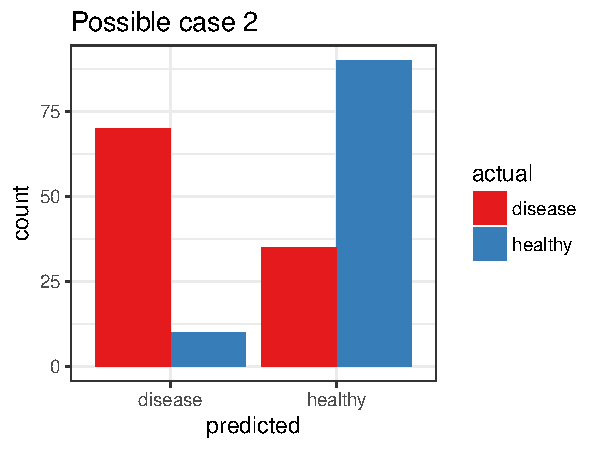
\includegraphics[width=0.33\textwidth]{images/meaningful_3}
	\end{center}
	
\end{frame}

\note{
	\begin{itemize}
		\item I want to begin with an introduction to the main question of my talk: 
		\item what makes a model \textsl{good} or \textsl{meaningful}?
	\end{itemize}
	
	\begin{enumerate}
		\item It answers a \textbf{specific} question or addresses a specific problem, \\
			e.g. does a mammogram image show a healthy breast or is there a tumor? \\
			Or does an ECG show a normal heart rhythm or arrhythmia?
		\item And it produces a correct outcome (e.g. a diagnosis) often enough that we trust it!
		\item And it needs to be generalizable, i.e. it needs to perform well on unseen data
	\end{enumerate}
	
	\begin{itemize}
		\item If we build models, we therefore need to evaluate its accuracy 
		\item before we can decide whether it is trustworthy enough to implement in real-life, 
		\item like in a hospital where it could e.g. assist doctors in making decisions on treatment
	\end{itemize}

	\begin{itemize}
		\item But what exactly is \textsl{high accuracy} can not be defined with a one-size-fits-all approach: 
		\item it depends on the problem we want to model. 	
	\end{itemize}
}

\note{
	Let me illustrate what I mean with the following examples:
	\begin{itemize}
		\item \alert{Ideal case:} Of course, we all want to achieve ideal modeling results where overall prediction accuracy is very high. \\ 
		With a model like that, we can be very confident that a healthy person is indeed healthy and a sick person is not. \\
		\item But in reality, we often achieve prediction accuracies that are much less nice. \\
		\item \alert{Scenarios 1 and 2:} Le's consider two possible scenarios: 
		\item in scenario 1, we can be very confident that a person who got classified as "healthy" is indeed healthy, \\ 
		while a person who has been diagnosed as diseased might as well be healthy based on these prediction accuracies
		\item in case 2, it is the other way around.
		\item We now need to make a decision which scenario is better and in which direction we want to optimize our model: \\ 
		do we rather want to refer a few healthy people for further checking because the model predicted them as diseased? \\ 
		Or do we rather want to be as certain as possible that a predicted disease is actually true \\ 
		and accept that we might miss a few disease cases?
	\end{itemize}
}

%%%%%%%%%%%%%%%%%%%%%
%	SECTION
%	Machine Learning (ML) in disease modeling
%%%%%%%%%%%%%%%%%%%%%

\section{Machine Learning (ML) in disease modeling}

\begin{frame}
	\frametitle{ML in disease modeling}
	
	\begin{itemize}
		\item tools that can interpret "big medical data" 
		\item and provide fast, accurate and actionable information
		\item for precision or personalized medicine
	\end{itemize}

	\vspace{0.5cm}

	\alert{Examples:} 
	\begin{itemize}
		\item computer-aided diagnosis of breast cancer \\ from mammograms\footcite{Kunio}
		\item identifying gene defects with facial recognition \\ software\footcite{Levenson}
		\item identifying signatures of Brain Cancer \\ from MRSI \footcite{doi:10.1146/annurev.bioeng.8.061505.095802}
		\item ... and many more ...
	\end{itemize}

	\begin{tikzpicture}[remember picture,overlay]
	\node[xshift=-2cm,yshift=4cm] at (current page.south east) {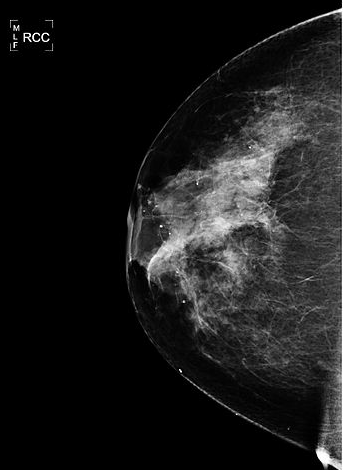
\includegraphics[width=3cm]{images/mammogram}};
	\end{tikzpicture}

	%\footfullcite{}
	
\end{frame}

\note{
	\begin{itemize}
		\item there is not a place in medicine where AI doesn't have potential applications:
		\item more data is being collected that needs to be interpretated
		\item increasingly data driven diagnosis, e.g. in radiology
		\item image recognition of e.g. tumors or pneumonia in medical images
		\item similar to training ML models to recognize images of cats (classification in images)
		\item ML allows incorporation of data from heterogenous inputs: 
		\item clinical, genomics, drugs, electronic health records, etc.
		\item = personalised medicine
	\end{itemize}

	\begin{itemize}
		\item A key aspect of precision medicine is the development of informatics tools 
		\item that can analyze and interpret 'big data' sets 
		\item in an automated and adaptive fashion 
		\item while providing accurate and actionable clinical information
		\item ML based models can improve detection, diagnosis, and therapeutic monitoring of disease
	\end{itemize}

	\begin{itemize}
		\item you can find things with ML that you wouldn't be able to find otherwise
		\item many models today perform better than humans!
		\item a patient with a rare difficult condition can be matched to similar cases from the past
		\item faster diagnosis, better treatment
	\end{itemize}
}

\note{	
	\begin{itemize}
		\item identifying breast cancer, lung cancer, osteoporosis, brain tumors, etc. from medical images
		\item predicting response of different cancer types to different treatments
		\item Computer-Aided Diagnosis (CAD) has become one of the major research subjects in medical imaging and diagnostic radiology
		\item With CAD, radiologists use the computer output as a 'second opinion' and make the final decisions
		\item In vivo magnetic resonance spectroscopy imaging (MRSI) allows noninvasive characterization 
		\item and quantification of molecular markers of potentially high clinical utility 
		\item for improving detection, identification, and treatment for a variety of diseases, most notably brain cancers
	\end{itemize}

	\begin{itemize}
		\item facial analysis technology aids diagnoses of genetic disorders
		\item researchers at the University of Oxford in the United Kingdom
		\item Face2Gene uses machine learning
		\item helps geneticists narrow down possible disorders that often involve dysmorphic facial features
	\end{itemize}

	\begin{itemize}
		\item doctors are still important!
		\item computer does the tasks that we humans are not good at, like interpreting complex images
		\item we have more data than humans can manage to make sense of (e.g. genomics data)
		\item the clinicians will be freed up to think about best treatment options and talk more with the patients
		\item good models are built on strong knowledge of the question and the biology behind it
		\item features need to be evaluated in context
	\end{itemize}
}

\begin{frame}[plain, c]
	
	\begin{center}
		\usebeamerfont*{frametitle} \usebeamercolor[fg]{frametitle} {\LARGE{the elephant in the room} \\ \vspace{0.5cm} \Huge{\textbf{Trust!}}}
	\end{center}
	
	\vspace{0.5cm}
	
	\begin{itemize}
		\item we don't know \alert{WHY} ML models make decisions
		\item inherent problem with ML models: \\ they are hard (or impossible) to interpret
	\end{itemize}

	\begin{itemize}
		\item therefore, it is crucial that our models are \alert{accurate} \\
				and \alert{meaningful}
	\end{itemize}
\end{frame}

\note{
	\begin{itemize}
		\item almost by definition one cannot really understand a good model.
		\item 
	\end{itemize}
}

%%%%%%%%%%%%%%%%%%%%%
%	SECTION
%	A quick recap of ML basics
%%%%%%%%%%%%%%%%%%%%%

\section{A quick recap of ML basics}

\begin{frame}
	\frametitle{Machine learning}

	\begin{itemize}
		\item artificial intelligence (AI)
		\item data-driven
		\item algorithms \alert{learn} by being trained on observed data...
		\item ... and \alert{predict unknown data}
		\item ML concepts are not new, but the increase in computational capacity has made them more accessible
	\end{itemize}
	
	\begin{block} {}	
		\begin{center}
			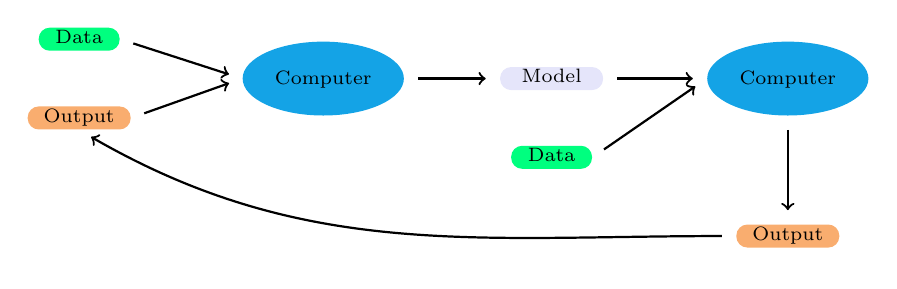
\begin{tikzpicture}
			\scriptsize
			\node[rectangle, rounded corners, text height=1ex,text depth=0ex,align=center,text width=3em,text centered,minimum height=1em, fill = SpringGreen] (Data) at (0,0) {Data};
			\node[rectangle, rounded corners, text height=1ex,text depth=0ex,align=center,text width=4em,text centered,minimum height=1em, fill = Lavender] (Model) at (6,-0.5) {Model};
			\node[ellipse, text height=3ex,text depth=1.5ex,align=center,text width=4.5em,text centered,minimum height=3em, fill = Cerulean] (Computer) at (3.1,-0.5) {Computer};
			\node[rectangle, rounded corners, text height=1ex,text depth=0ex,align=center,text width=4em,text centered,minimum height=1em, fill = Apricot] (Output) at (0,-1) {Output};
			\node[ellipse, text height=3ex,text depth=1.5ex,align=center,text width=4.5em,text centered,minimum height=3em, fill = Cerulean] (Computer2) at (9,-0.5) {Computer};
			\node[rectangle, rounded corners, text height=1ex,text depth=0ex,align=center,text width=4em,text centered,minimum height=1em, fill = Apricot] (Output2) at (9,-2.5) {Output};
			\node[rectangle, rounded corners, text height=1ex,text depth=0ex,align=center,text width=3em,text centered,minimum height=1em, fill = SpringGreen] (Data2) at (6,-1.5) {Data};
			
			\draw[->,thick,shorten >=5pt,shorten <=5pt] (Data.east) -- (Computer.west);
			\draw[->,thick,shorten >=5pt,shorten <=5pt] (Output.east) -- (Computer.west);
			\draw[->,thick,shorten >=5pt,shorten <=5pt] (Computer.east) -- (Model.west);
			\draw[->,thick,shorten >=5pt,shorten <=5pt] (Model.east) -- (Computer2.west);
			\draw[->,thick,shorten >=5pt,shorten <=5pt] (Computer2.south) -- (Output2.north);
			\draw[->,thick,shorten >=5pt,shorten <=5pt] (Data2.east) -- (Computer2.west);
			\draw[->,thick,shorten >=5pt,shorten <=5pt] (Output2.west) to [out=180,in=330] (Output.south);
			\end{tikzpicture}
		\end{center}
	\end{block}
\end{frame}

\begin{frame}
	\frametitle{Supervised vs Unsupervised algorithms}

	\begin{columns}
		
		\column{0.5\textwidth}
	
	\begin{block}{}
		\centering
		\alert{Supervised}
	\end{block}

	\begin{center}
		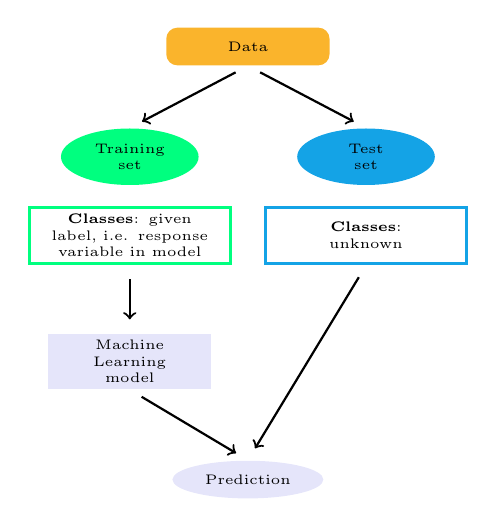
\begin{tikzpicture}
		\tiny
		\node[rectangle, rounded corners, align=center,text width=8em,text centered,minimum height=2em, fill = Dandelion] (select) at (2.5,-3) {Data};
		
		\node[ellipse,align=center,text width=4.5em,text centered,minimum height=3em, fill = SpringGreen] (training) at (1,-4.4) {Training set};
		
		\node[rectangle, align=center,text width=10em,text centered,minimum height=3em, draw = SpringGreen, very thick] (class1) at (1,-5.4) {\textbf{Classes}: given label, i.e. response variable in model};
		
		\node[ellipse,align=center,text width=4.5em,text centered,minimum height=3em, fill = Cerulean] (test) at (4,-4.4) {Test \\ set};
		
		\node[rectangle, align=center,text width=10em,text centered,minimum height=3em, draw = Cerulean, very thick] (class2) at (4,-5.4) {\textbf{Classes}: \\ unknown};
		
		\node[rectangle, align=center,text width=8em,text centered,minimum height=2em, fill = Lavender] (rf) at (1,-7.0) {Machine \\ Learning \\ model};
		
		\node[ellipse,align=center,text width=5em,text centered,minimum height=2em, fill = Lavender] (prediction) at (2.5,-8.5) {Prediction};
		
		\draw[->,thick,shorten >=5pt,shorten <=5pt] (select.south) -- (training.north);
		\draw[->,thick,shorten >=5pt,shorten <=5pt] (select.south) -- (test.north);
		
		\draw[->,thick,shorten >=5pt,shorten <=5pt] (class1.south) -- (rf.north);
		\draw[->,thick,shorten >=5pt,shorten <=5pt] (class2.south) -- (prediction.north);
		
		\draw[->,thick,shorten >=5pt,shorten <=5pt] (rf.south) -- (prediction.north);
		\end{tikzpicture}
	\end{center}

	\column{0.5\textwidth}
	
	\begin{block}{}
		\centering
		\alert{Unsupervised}
	\end{block}

	\centering
	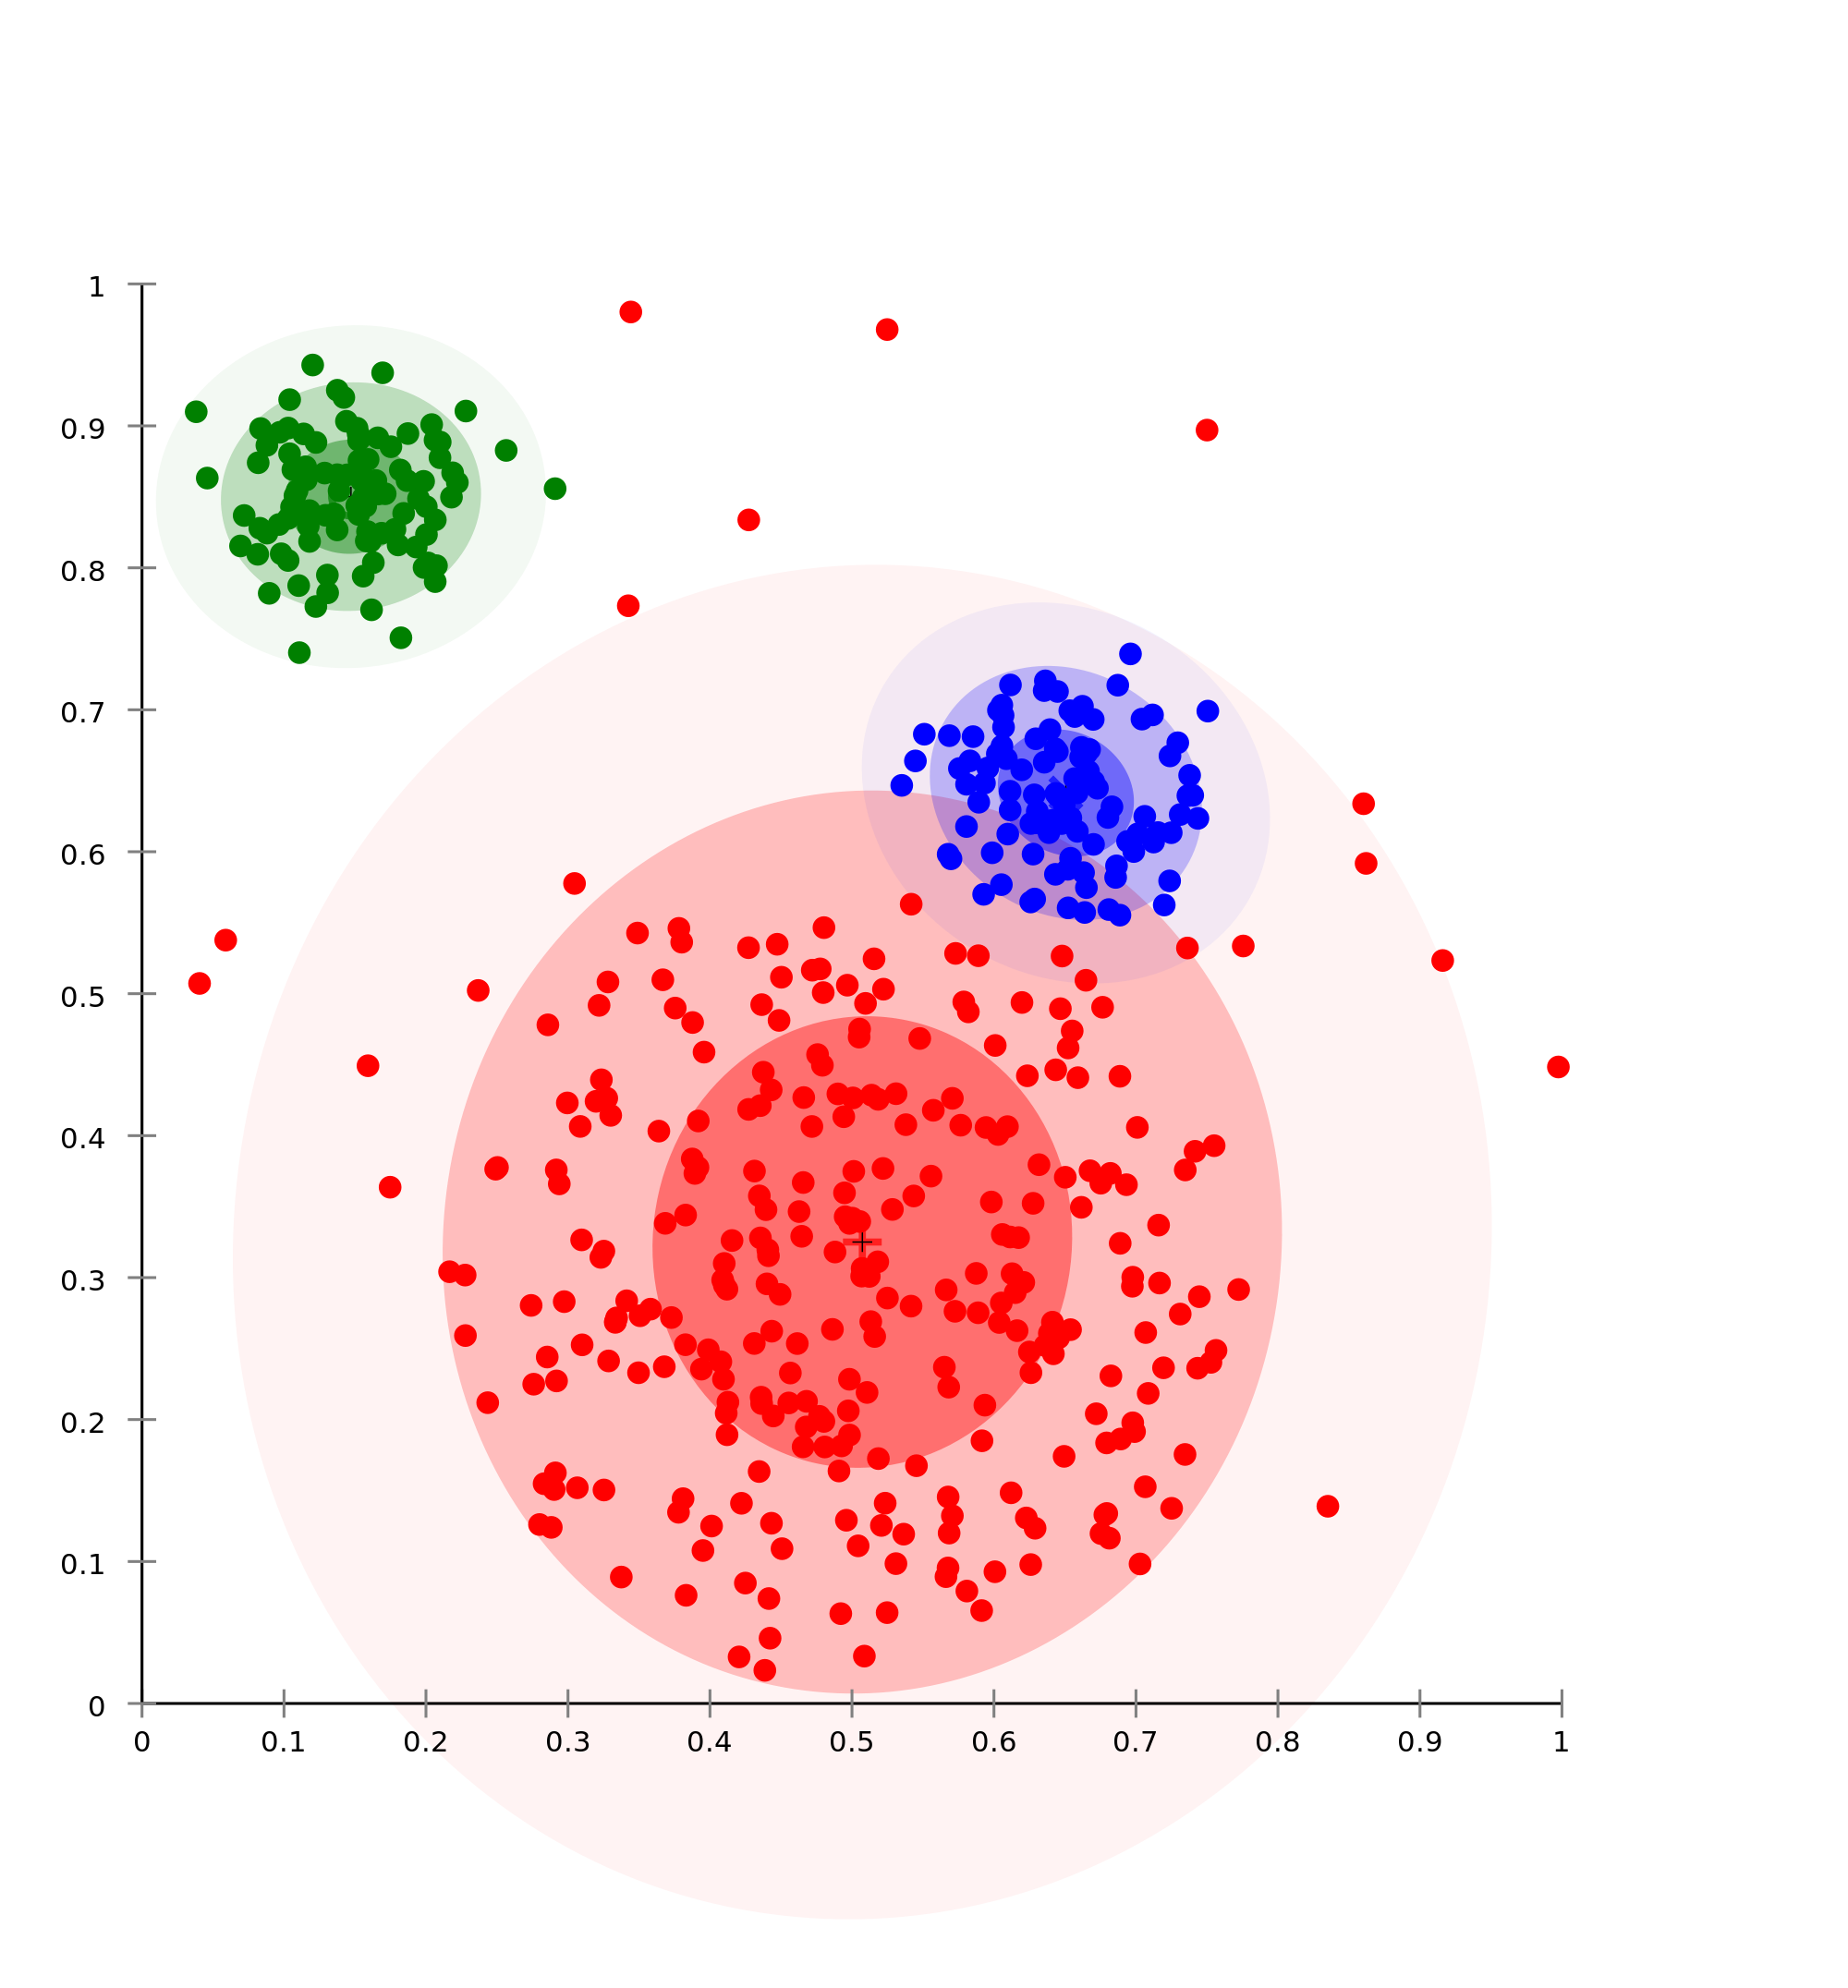
\includegraphics[width=0.5\textwidth]{images/clustering1}
	
	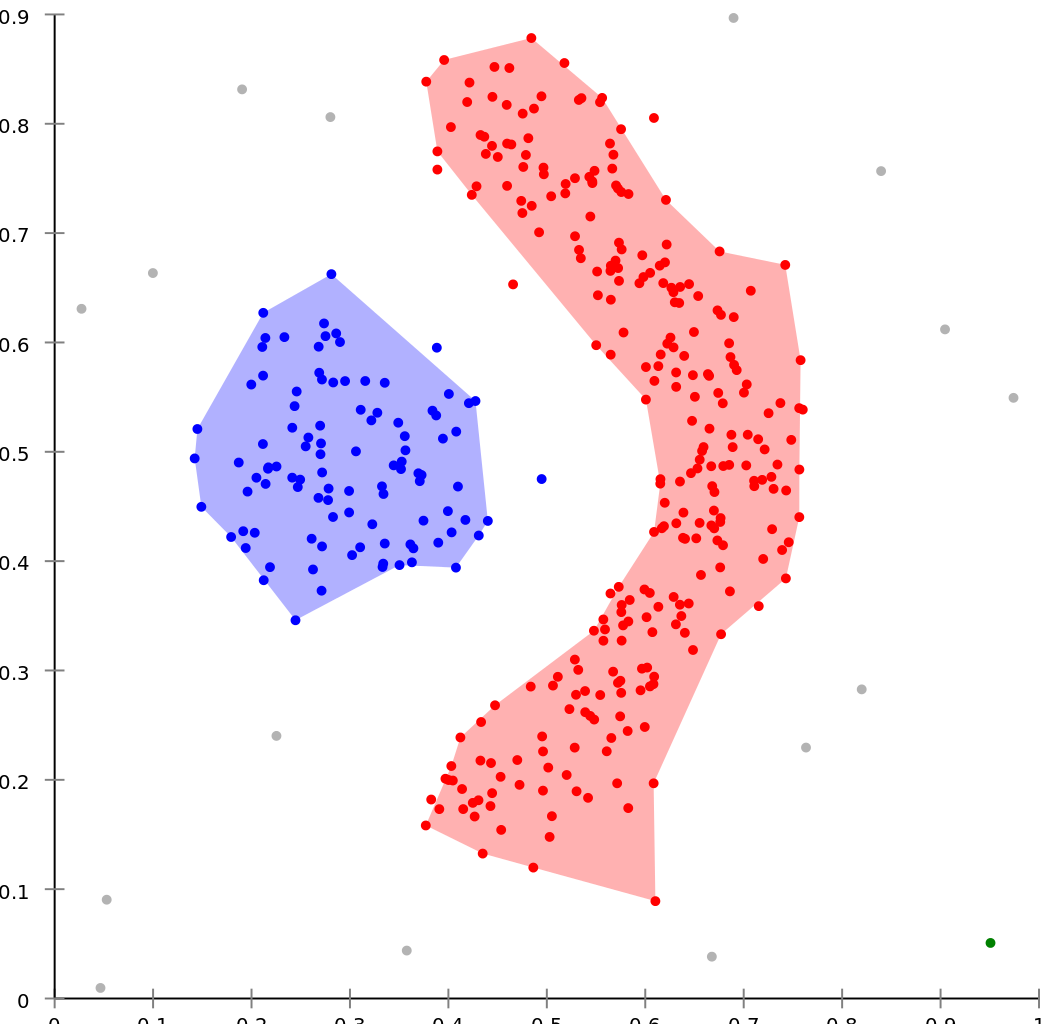
\includegraphics[width=0.5\textwidth]{images/clustering2}
	
	\end{columns}
\end{frame}

\note{
	\begin{itemize}
		\item Unsupervised:
		\item no input!
		\item matrix decomposition methods, e.g. nonnegative matrix factorization
		\item pattern recognition
		\item clusters data into different groups
		\item able to recover biomarkers of disease and toxicity
	\end{itemize}

	\begin{itemize}
		\item Supervised
		\item classification labels are given
		\item e.g. support vector machine
	\end{itemize}

	\begin{itemize}
	\item Semi-supervised:
	\item a little bit of input, like how many classes to find
	\end{itemize}

	Here, I will focus on supervised learning!
}


\begin{frame}
	\frametitle{Classification vs Regression}

		\begin{columns}
		
		\column{0.5\textwidth}
		
		\begin{block}{}
			\centering
			\alert{Classification} \\
			e.g. healthy vs disease
		\end{block}
		
		\begin{center}
			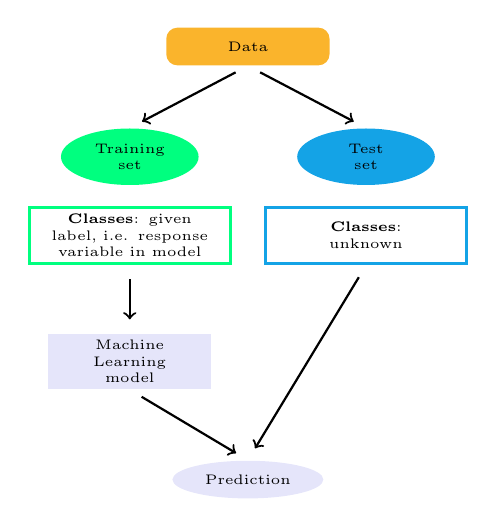
\begin{tikzpicture}
			\tiny
			\node[rectangle, rounded corners, align=center,text width=8em,text centered,minimum height=2em, fill = Dandelion] (select) at (2.5,-3) {Data};
			
			\node[ellipse,align=center,text width=4.5em,text centered,minimum height=3em, fill = SpringGreen] (training) at (1,-4.4) {Training set};
			
			\node[rectangle, align=center,text width=10em,text centered,minimum height=3em, draw = SpringGreen, very thick] (class1) at (1,-5.4) {\textbf{Classes}: given label, i.e. response variable in model};
			
			\node[ellipse,align=center,text width=4.5em,text centered,minimum height=3em, fill = Cerulean] (test) at (4,-4.4) {Test \\ set};
			
			\node[rectangle, align=center,text width=10em,text centered,minimum height=3em, draw = Cerulean, very thick] (class2) at (4,-5.4) {\textbf{Classes}: \\ unknown};
			
			\node[rectangle, align=center,text width=8em,text centered,minimum height=2em, fill = Lavender] (rf) at (1,-7.0) {Machine \\ Learning \\ model};
			
			\node[ellipse,align=center,text width=5em,text centered,minimum height=2em, fill = Lavender] (prediction) at (2.5,-8.5) {Prediction};
			
			\draw[->,thick,shorten >=5pt,shorten <=5pt] (select.south) -- (training.north);
			\draw[->,thick,shorten >=5pt,shorten <=5pt] (select.south) -- (test.north);
			
			\draw[->,thick,shorten >=5pt,shorten <=5pt] (class1.south) -- (rf.north);
			\draw[->,thick,shorten >=5pt,shorten <=5pt] (class2.south) -- (prediction.north);
			
			\draw[->,thick,shorten >=5pt,shorten <=5pt] (rf.south) -- (prediction.north);
			\end{tikzpicture}
		\end{center}
		
		\column{0.5\textwidth}
		
		\pause
		
		\begin{block}{}
			\centering
			\alert{Regression} \\
			e.g. weight loss
		\end{block}
		
		\begin{center}
			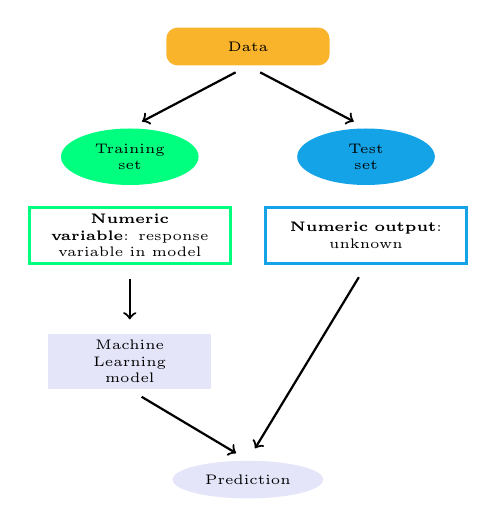
\begin{tikzpicture}
			\tiny
			\node[rectangle, rounded corners, align=center,text width=8em,text centered,minimum height=2em, fill = Dandelion] (select) at (2.5,-3) {Data};
			
			\node[ellipse,align=center,text width=4.5em,text centered,minimum height=3em, fill = SpringGreen] (training) at (1,-4.4) {Training set};
			
			\node[rectangle, align=center,text width=10em,text centered,minimum height=3em, draw = SpringGreen, very thick] (class1) at (1,-5.4) {\textbf{Numeric \\ variable}: response variable in model};
			
			\node[ellipse,align=center,text width=4.5em,text centered,minimum height=3em, fill = Cerulean] (test) at (4,-4.4) {Test \\ set};
			
			\node[rectangle, align=center,text width=10em,text centered,minimum height=3em, draw = Cerulean, very thick] (class2) at (4,-5.4) {\textbf{Numeric output}: \\ unknown};
			
			\node[rectangle, align=center,text width=8em,text centered,minimum height=2em, fill = Lavender] (rf) at (1,-7.0) {Machine \\ Learning \\ model};
			
			\node[ellipse,align=center,text width=5em,text centered,minimum height=2em, fill = Lavender] (prediction) at (2.5,-8.5) {Prediction};
			
			\draw[->,thick,shorten >=5pt,shorten <=5pt] (select.south) -- (training.north);
			\draw[->,thick,shorten >=5pt,shorten <=5pt] (select.south) -- (test.north);
			
			\draw[->,thick,shorten >=5pt,shorten <=5pt] (class1.south) -- (rf.north);
			\draw[->,thick,shorten >=5pt,shorten <=5pt] (class2.south) -- (prediction.north);
			
			\draw[->,thick,shorten >=5pt,shorten <=5pt] (rf.south) -- (prediction.north);
			\end{tikzpicture}
		\end{center}
		
	\end{columns}
\end{frame}

\note{
	\begin{itemize}
		\item Supervised learning!
		\item Your learning algorithm seeks a function from inputs to the respective targets. 
		\item If the targets are expressed in some classes, it is called classification problem. 
		\item Alternatively, if the target space is continuous, it is called regression problem.
	\end{itemize}
}


\begin{frame}
	\frametitle{Features}
	
	Features are the variables used for model training. \\
	Using the right features is crucial.
	
		\vspace{0.5cm}

	\alert{More is not necessarily better (overfitting)!}
	
		\vspace{0.5cm}

	\begin{itemize}
		\item feature selection
		\item feature extraction/ engineering
	\end{itemize}
\end{frame}

\note{
	Machine learning uses so called features (i.e. variables or attributes) to generate predictive models. Using a suitable combination of features is essential for obtaining high precision and accuracy. Because too many (unspecific) features pose the problem of overfitting the model, we generally want to restrict the features in our models to those, that are most relevant for the response variable we want to predict. Using as few features as possible will also reduce the complexity of our models, which means it needs less time and computer power to run and is easier to understand. \\

	extraction of salient structure in the data that is more informative than the raw data itself (the feature extraction problem)
}

\begin{frame}
	\frametitle{Training, (cross-) validation and test data}
	
\end{frame}

\note{
	Decide cross validation strategy - To avoid overfitting, make sure you've set up a cross validation strategy in early stages. A nice CV strategy will help you get reliable score on leaderboard.
	
	preventing overfitting, we want our models to be generalizable
	
	Cross validation means that from my main set, I create RANDOMLY 2 sets. I built (train) my algorithm with the first one (let?s call it training set) and score the other (let?s call it validation set). I repeat this process multiple times and always check how my model performs on the test set in respect to the metric I want to optimize.
	
	The process may look like:
	
	For 10 (you choose how many X) times
	Split the set in training (50%-90% of the original data)
	And validation (50%-10%  of the original data)
	Then fit the algorithm on the training set
	Score the validation set.
	Save the result of that scoring in respect to the chosen metric.
	Calculate the average of these 10 (X) times. That how much you expect this score in real life and is generally a good estimate.
	Remember to use a SEED to be able to replicate these X splits
	Other things to consider is Kfold and stratified KFold . Read here. For time sensitive data, make certain you always the rule of having past predicting future when testings.
}
\begin{frame}
	\frametitle{Hyper Parameter Tuning}
	
\end{frame}

\note{
	Grid Search
	
	Start hyper parameter tuning - Once CV is at place, try improving model's accuracy using hyper parameter tuning. It further includes the following steps:
	Data transformations: It involve steps like scaling, removing outliers, treating null values,  transform categorical variables, do feature selections, create interactions etc.
	Choosing algorithms and tuning their hyper parameters: Try multiple algorithms to understand how model performance changes.
	Saving results: From all the models trained above, make sure you save their predictions. They will be useful for ensembling.
	Combining models: At last, ensemble the models, possibly on multiple levels. Make sure the models are correlated for best results.
}

\begin{frame}[plain, c]
	
	\begin{center}
	\usebeamerfont*{frametitle} \usebeamercolor[fg]{frametitle} {\Huge \textbf{Take home messages:}}
	\end{center}

	\vspace{0.5cm}

	\begin{itemize}
		\item ...
	\end{itemize}
\end{frame}

%%%%%%%%%%%%%%%%%%%%%
%	SECTION
%	How to build ML models in R
%%%%%%%%%%%%%%%%%%%%%

\section{How to build ML models in R}

\begin{frame}
	\frametitle{Session setup}
	
	\begin{itemize}
		\item RStudio
		\item Breast Cancer Wisconsin Dataset
		\item caret\footfullcite{caret}
		\item h2o\footfullcite{h2o}
	\end{itemize}
	
	\vspace{0.5cm}
	
	\centering
	Code will be available on \href{https://shiring.github.io}{my website} and on \href{https://github.com/ShirinG/Webinar_ML_for_disease}{Github}
	
	\begin{tikzpicture}[remember picture,overlay]
	\node[xshift=-2.3cm,yshift=-2.3cm] at (current page.north east) {
\includegraphics[width=3cm]{images/R_logo.png}};
	\end{tikzpicture}
	
\end{frame}

\begin{frame}
	\frametitle{Get to know your data}
	
	\alert{Response variable}
	\begin{itemize}
		\item Is it balanced?
	\end{itemize}
	
	\begin{columns}	
		\column{0.5\textwidth}
		\centering
		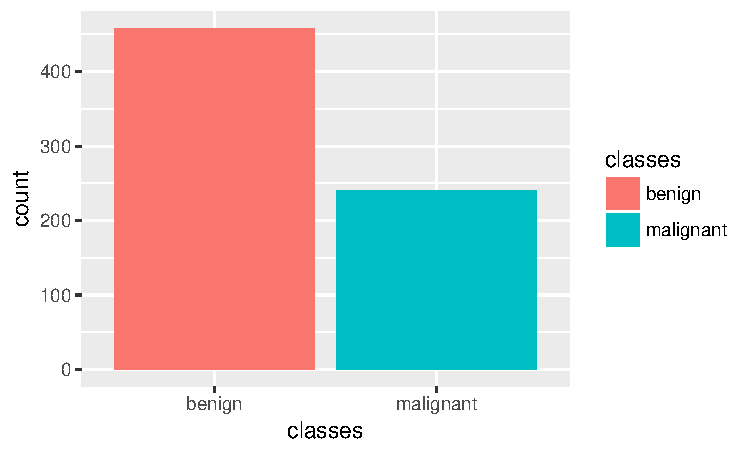
\includegraphics[width=0.9\textwidth]{webinar_code_files/figure-latex/response_classification-1.pdf}
		
		\column{0.5\textwidth}
		\centering
		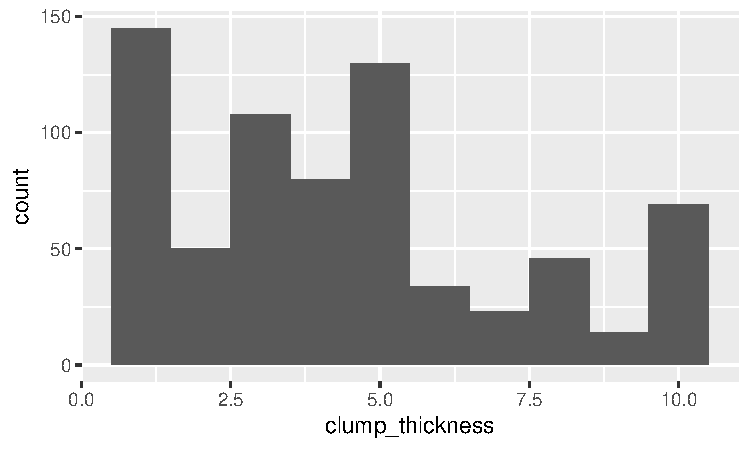
\includegraphics[width=0.9\textwidth]{webinar_code_files/figure-latex/response_regression-1.pdf}
	\end{columns}
	
		\vspace{0.5cm}

	\alert{Missing data}
	\begin{itemize}
		\item Is there missing data?
		\item Can we afford to loose data points with missing values?
		\item Or do we use imputation (and introduce additional uncertainty)?
	\end{itemize}

\end{frame}

\note{
	\begin{itemize}
		\item Understand the data
		\item Look at data types. 
		\item Check variable classes. 
		\item Create some univariate - bivariate plots to understand the nature of variables.
		\item Most important to know is the distribution: are the classes balanced?
		\item If we have unbalanced data, this will effect our model later on \\
		We would have to consider over- or undersampling.
	\end{itemize}

	\begin{itemize}
		\item Missing data
		\item If we have lots of data and few missing values, we can afford to loose these data points.
		\item If we don't have that much data though, our model will probably loose significant power if we remove the samples.
		\item In that case, we would rather introduce a certain uncertainty by imputing missing values. 
	\end{itemize}	
}

\begin{frame}
	\frametitle{Get to know your data}
	\alert{Principal Component Analysis (PCA)}
	
	\vspace{0.5cm}

	\centering
	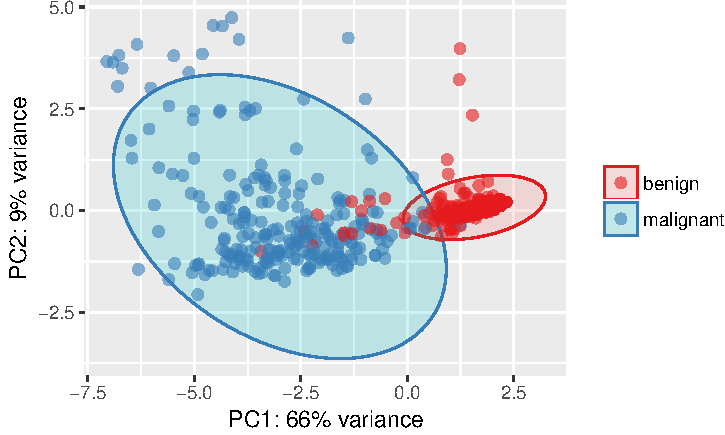
\includegraphics[width=0.9\textwidth]{webinar_code_files/figure-latex/pca-1.pdf}
\end{frame}

\begin{frame}
	\frametitle{Get to know your data}
	\alert{Principal Component Analysis (PCA)}
	
	\vspace{0.5cm}

	\centering
	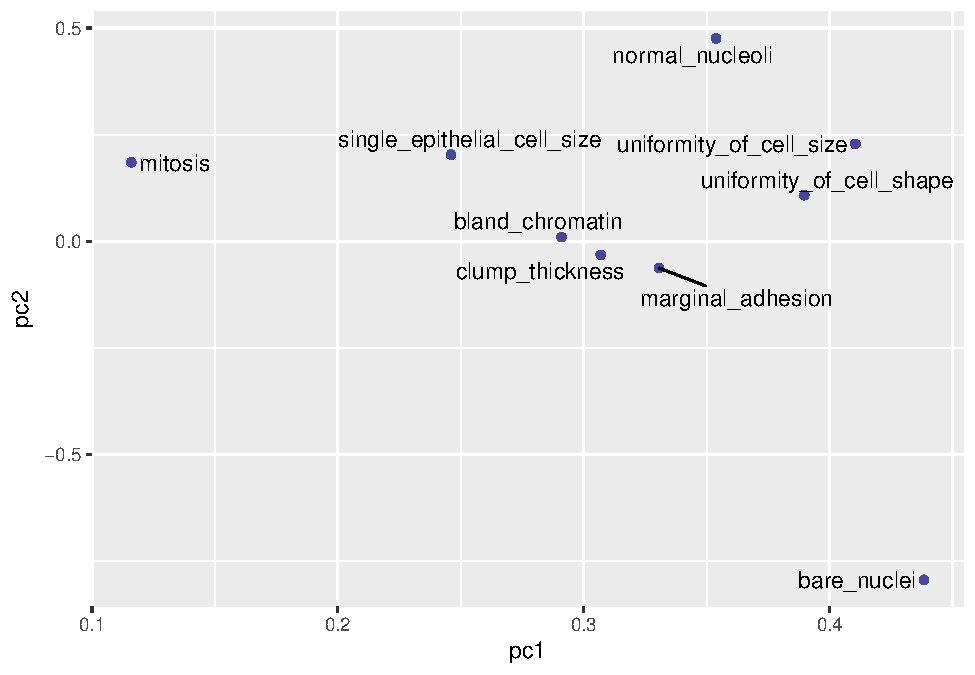
\includegraphics[width=0.8\textwidth]{webinar_code_files/figure-latex/pca_features-1.pdf}
\end{frame}

\note{
	\begin{itemize}
		\item To get an idea about the dimensionality and variance of the datasets, I am first looking at PCA plots
		\item for samples and features
		\item The first two principal components (PCs) show the two components that explain the majority of variation in the data
	\end{itemize}
}

\begin{frame}
	\frametitle{Get to know your data}
	\alert{Features}
	
	\begin{itemize}
		\item factors or numeric
		\item pre-processing
	\end{itemize}
	
	\centering
	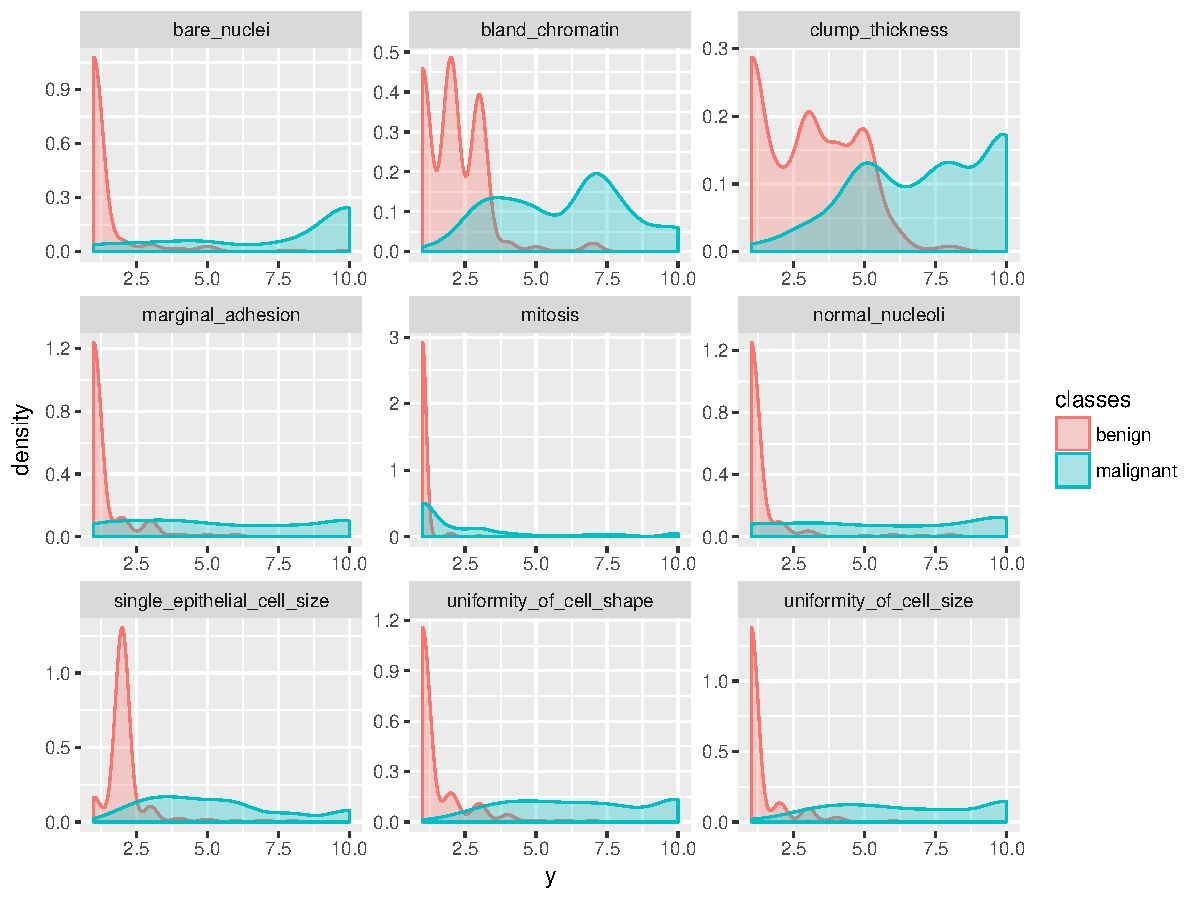
\includegraphics[width=0.7\textwidth]{webinar_code_files/figure-latex/features-1.pdf}
\end{frame}

\begin{frame}
	\frametitle{Get to know your data}
	\alert{Correlation}

	\centering
	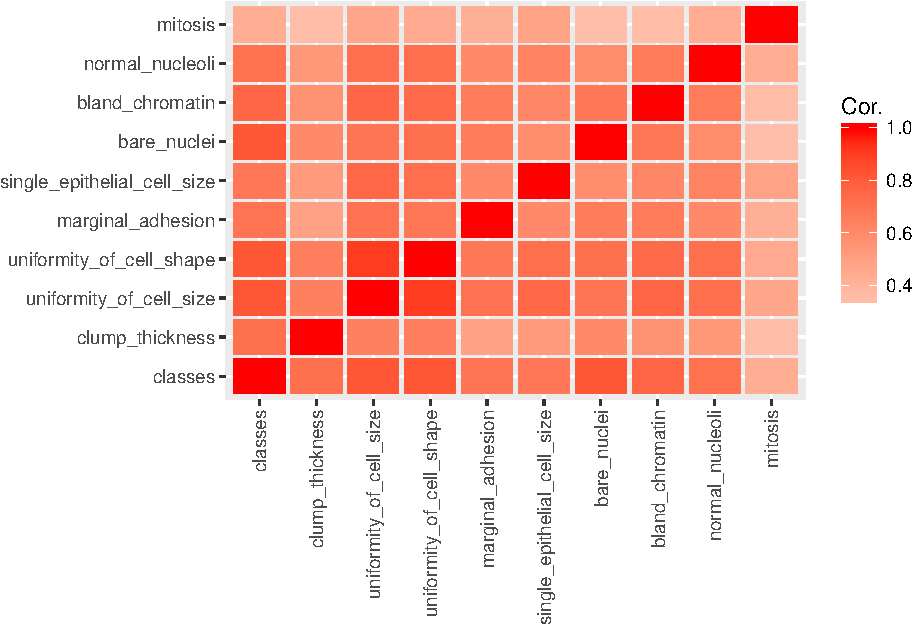
\includegraphics[width=0.9\textwidth]{webinar_code_files/figure-latex/corr_plot-1.pdf}
\end{frame}

\begin{frame}
	\frametitle{Training, validation and test data}
	
	We need to split the data into training and test sets - \\
	ideally \alert{stratified} by response class.
	
	\vspace{0.5cm}

	\alert{Density distribution}
	\begin{center}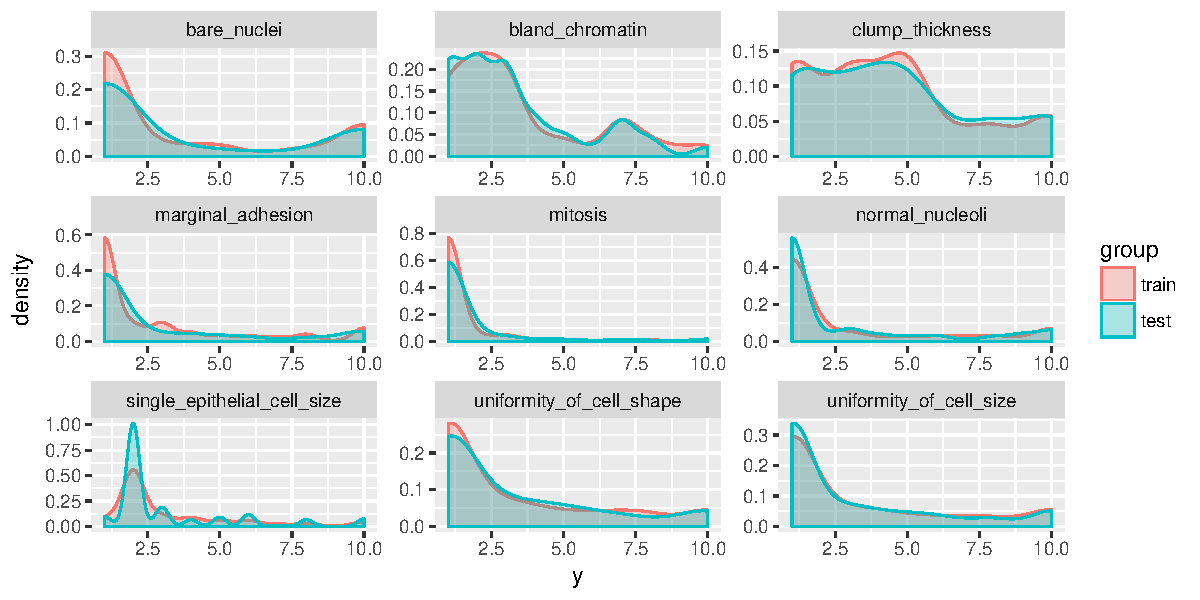
\includegraphics[width=1\textwidth]{webinar_code_files/figure-latex/distribution-1} \end{center}
\end{frame}

\note{
	For accurate predictions, density distribution should be similar in training and test data!
}

\begin{frame}
	\frametitle{Classification with tree-based models}
	\alert{Decision trees} \\ e.g. Random Forest and gradient boosting trees
		
	\begin{center}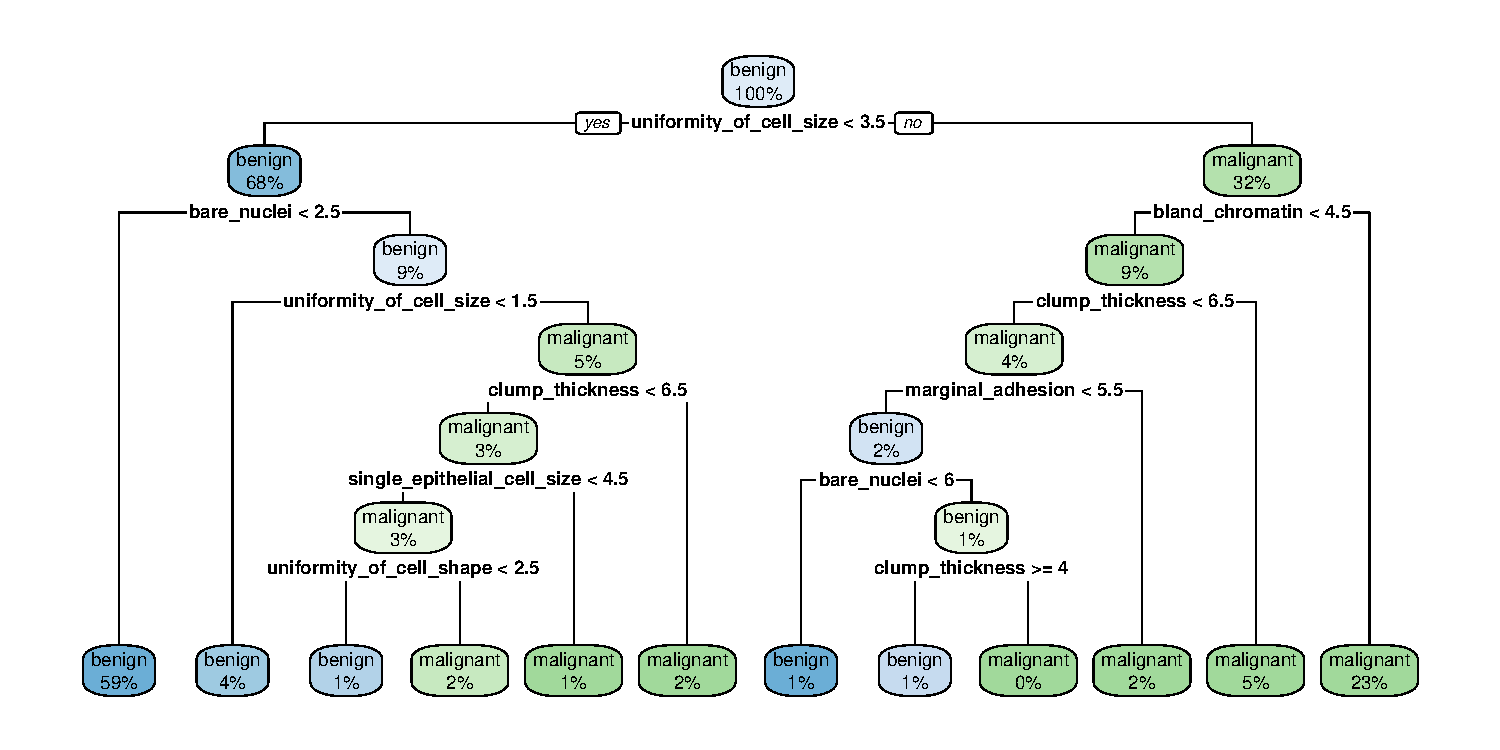
\includegraphics[width=1\textwidth]{webinar_code_files/figure-latex/decision_tree-1} \end{center}

\end{frame}

\note{
	\begin{itemize}
		\item We start with a group of samples
		\item for each sample, we assign a class: e.g. it comes from a benign or malignant tumor
		\item for each sample, we also have a number of features
		\item a decision trees separates the data at several nodes to end up with classifications at the final leaves
		\item the model learns a conditional structure of discriminative features
	\end{itemize}

	\begin{itemize}
		\item Random Forests produces multiple decision trees
		\item with some level of randomness
		\item each tree is evaluated regarding how well it classified the samples (cross-validation)
		\item if two trees are equally accurate, the tree with fewer nodes is preferred
		\item 'information gain' is the measure that tells us how good a tree model is
		\item better generalization than individual trees
	\end{itemize}
}

\begin{frame}[fragile]
	\frametitle{Tree-based classification}
	
	\begin{itemize}
		\item \alert{Random Forest or Gradient boosting}
		\item  with \textsl{caret}\footfullcite{caret}
	\end{itemize}

	\centering
	\begin{Verbatim}[fontsize=\footnotesize]
caret::train(classes ~ .,
             data = train_data,
             method = "rf",  # or "xgb"
             preProcess = c("scale", "center"),
             trControl = trainControl(method = "repeatedcv", 
                                      number = 10, 
                                      repeats = 10, 
                                      savePredictions = TRUE, 
                                      verboseIter = FALSE))
                                      
##           benign malignant class.error
## benign       313         8  0.02492212
## malignant      4       165  0.02366864
	\end{Verbatim}

\end{frame}

\note{
This function sets up a grid of tuning parameters for a number of classification and regression routines, fits each model and calculates a resampling based performance measure.

train can be used to tune models by picking the complexity parameters that are associated with the optimal resampling statistics. For particular model, a grid of parameters (if any) is created and the model is trained on slightly different data for each candidate combination of tuning parameters. Across each data set, the performance of held-out samples is calculated and the mean and standard deviation is summarized for each combination. The combination with the optimal resampling statistic is chosen as the final model and the entire training set is used to fit a final model.

The predictors in x can be most any object as long as the underlying model fit function can deal with the object class. The function was designed to work with simple matrices and data frame inputs, so some functionality may not work (e.g. pre-processing). When using string kernels, the vector of character strings should be converted to a matrix with a single column.
}

\begin{frame}
	\frametitle{Feature importance}
	
	\begin{center}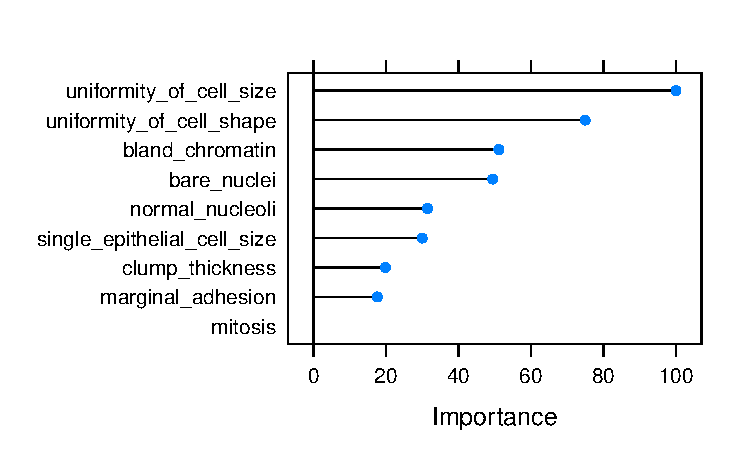
\includegraphics[width=0.8\textwidth]{webinar_code_files/figure-latex/importance_rf-1.pdf} \end{center}
\end{frame}

\note{
	Not all of the features I created will be equally important to the model. The decision tree already gave me an idea of which features might be most important but I also want to estimate feature importance using a Random Forest approach with repeated cross validation.

}


\begin{frame}
	\frametitle{Regression with (Generalized) Linear Models}
	
\end{frame}

\subsubsection{}


\begin{frame}
	\frametitle{Deep learning with neural networks}
	
	\begin{itemize}
		\item for BIG data
		\item with \textsl{h2o}\footfullcite{h2o}
	\end{itemize}
	
	\alert{Grid Search}
\end{frame}

%%%%%%%%%%%%%%%%%%%%%
%	SECTION
%	Evaluating model performance
%%%%%%%%%%%%%%%%%%%%%

\section{Evaluating model performance}

\begin{frame}
	\frametitle{Area Under the Curve (AUC}
	
	\centering
	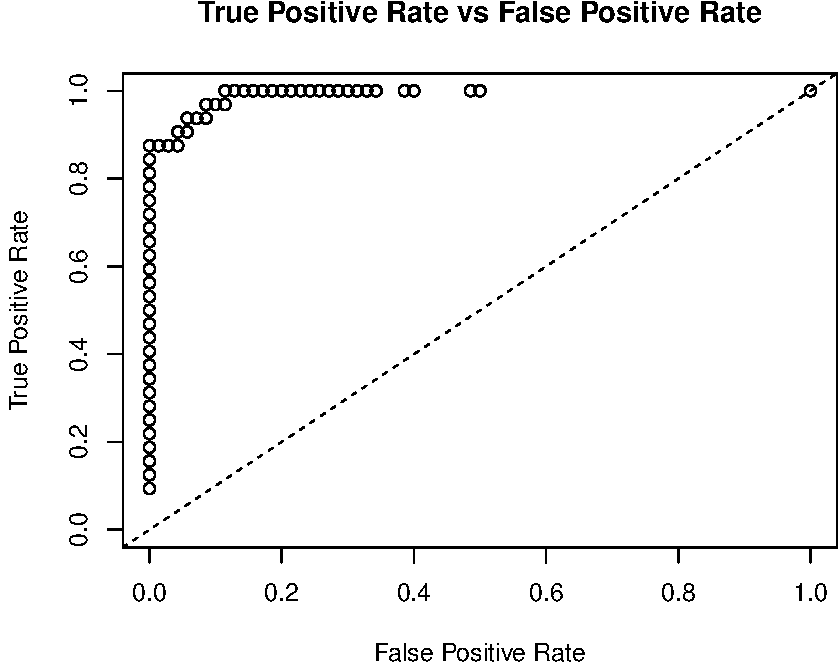
\includegraphics[width=0.8\textwidth]{webinar_code_files/figure-latex/auc_curve-1.pdf} 
\end{frame}

\begin{frame}
	\frametitle{AUC and mean squared error (MSE)}
	
	\begin{center}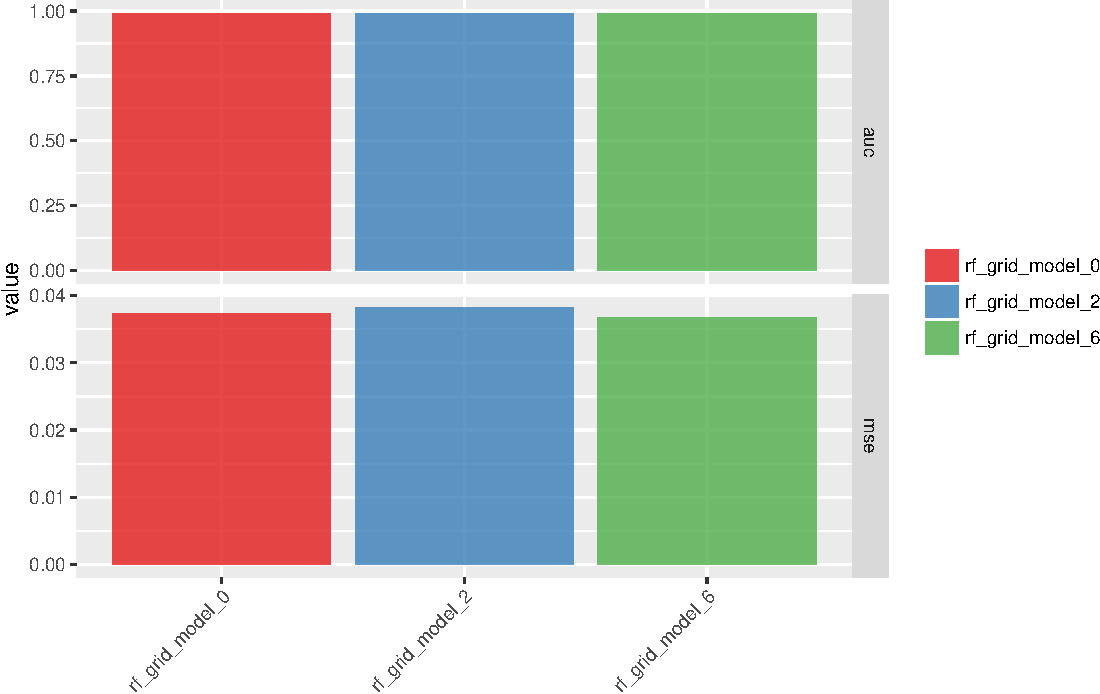
\includegraphics[width=1\textwidth]{webinar_code_files/figure-latex/auc_mse-1.pdf} \end{center}
\end{frame}

\begin{frame}
	\frametitle{Predictions on test data}
	\alert{Classification}
	
	\begin{columns}
	\column{0.5\textwidth}
	
	\centering
	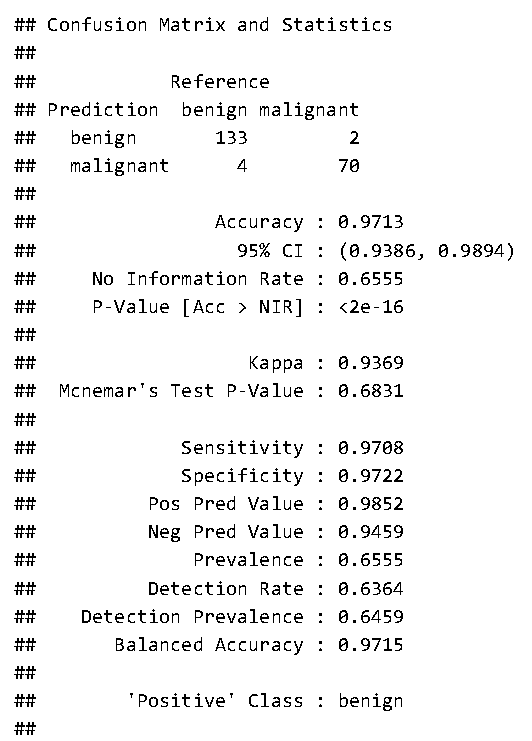
\includegraphics[width=0.9\textwidth]{images/results_matrix.pdf}
	
	\column{0.5\textwidth}
	\centering	
	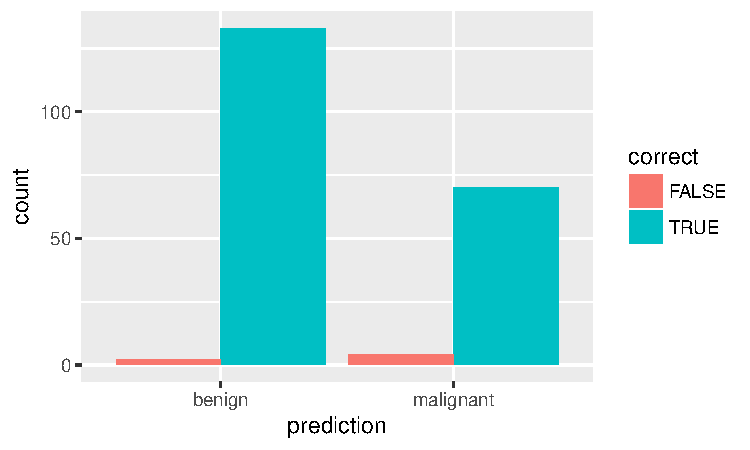
\includegraphics[width=1\textwidth]{webinar_code_files/figure-latex/results_bar_rf-1.pdf}
	
	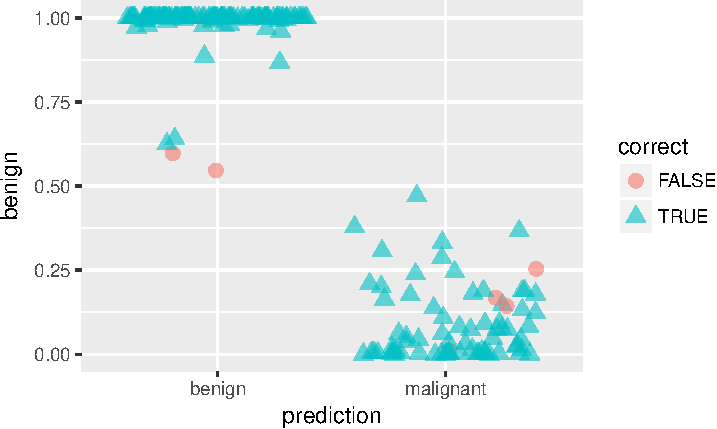
\includegraphics[width=1\textwidth]{webinar_code_files/figure-latex/results_jitter_rf-1.pdf} 
\end{columns}\end{frame}

\begin{frame}
	\frametitle{Predictions on test data}
	
	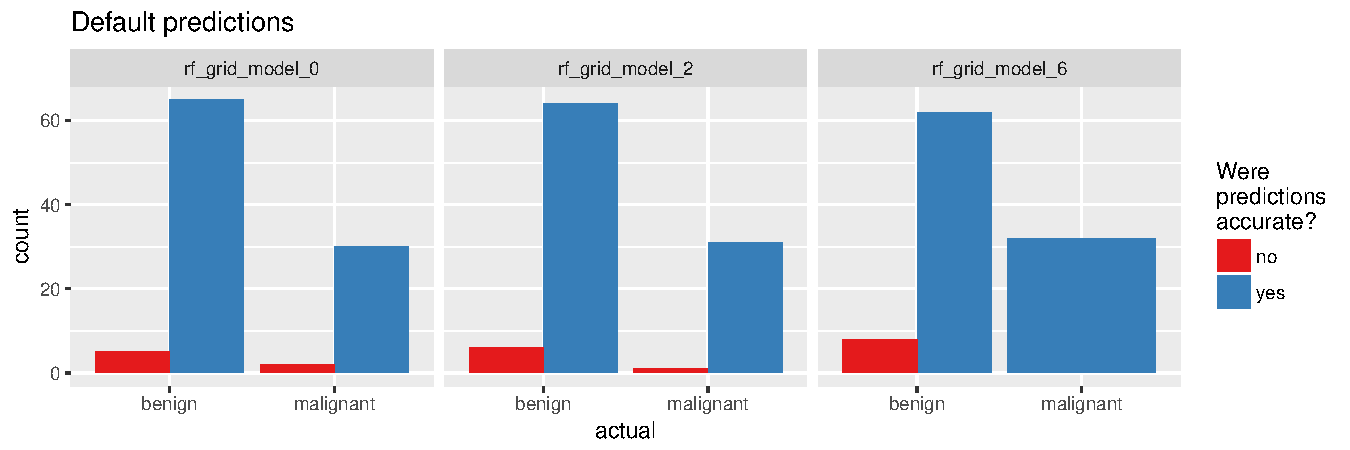
\includegraphics[width=1\textwidth]{webinar_code_files/figure-latex/final_predictions_rf-1.pdf} 

	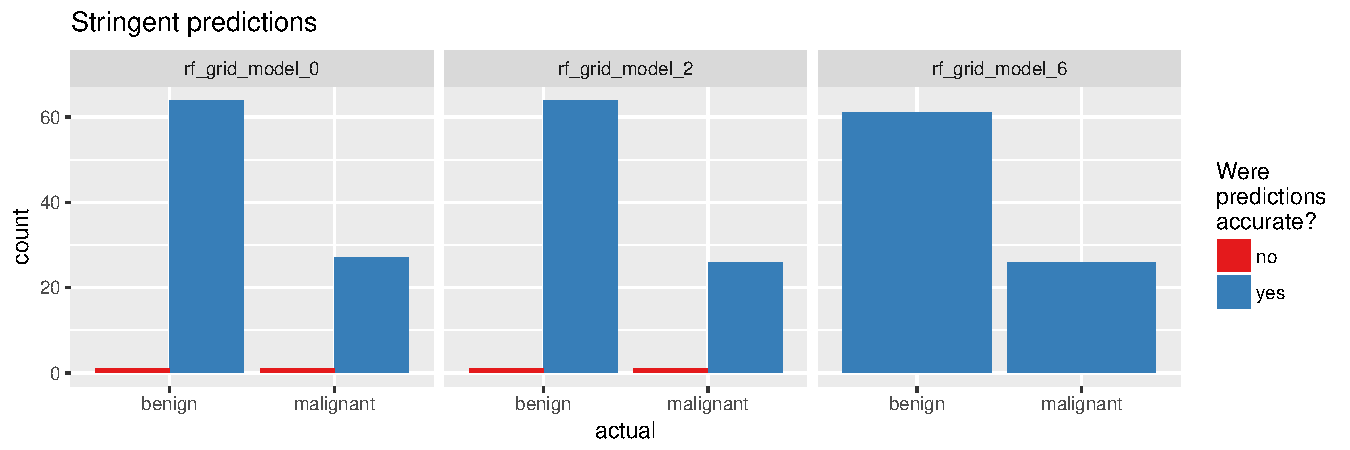
\includegraphics[width=1\textwidth]{webinar_code_files/figure-latex/final_predictions_rf-2.pdf} 
\end{frame}


\begin{frame}
	\frametitle{Predictions on test data}
	\alert{Regression}
	
	\begin{itemize}
		\item RMSE: 1.974296
		\item Rsquared: 0.5016141
	\end{itemize}
	
	\centering
	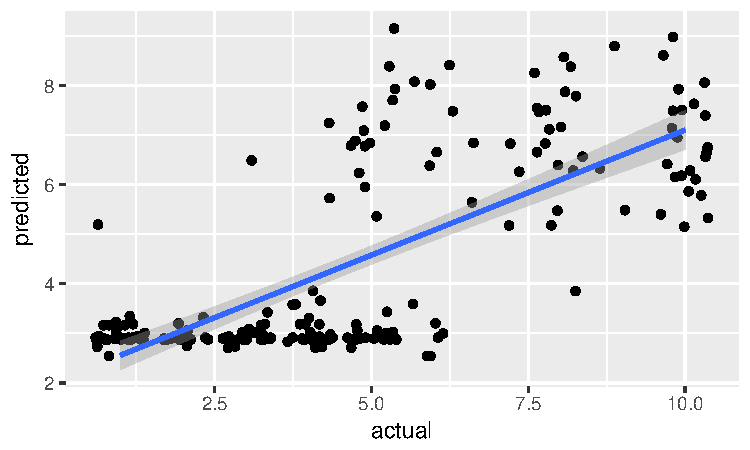
\includegraphics[width=0.8\textwidth]{webinar_code_files/figure-latex/regression_result-1.pdf}
\end{frame}


% accuracy
% Kappa

\begin{frame}[plain, c]
	
	\begin{center}
		\usebeamerfont*{frametitle} \usebeamercolor[fg]{frametitle} {\Huge \textbf{Take home messages:}}
	\end{center}
	
	\vspace{0.5cm}
	
	\begin{itemize}
		\item ...
	\end{itemize}
\end{frame}

\begin{frame}
	\frametitle{Outlook}
	
	\begin{itemize}
		\item `big data' needs to be big!
		\item for really meaningful models, data needs to be shared
		\item the more data, the more accurate and generalizable the models will be
		\item issues: privacy, platform, quality standards
		\item ML could make health care more cost-effective by reducing the energy required for interpretation
	\end{itemize}
\end{frame}

%%%%%%%%%%%%%%%%%%%%%

\begin{frame}[plain, c]
	
	\begin{center}
	\usebeamerfont*{frametitle} \usebeamercolor[fg]{frametitle} {\Huge \textbf{Thank you for your attention!}}
	\end{center}

	\vspace{0.5cm}

	\begin{center}
		\usebeamerfont*{frametitle} {\huge Questions?}
	\end{center}

	\vspace{0.5cm}
	
	Slides and code will be available on Github: \href{https://github.com/ShirinG/Webinar_ML_for_disease}{https://github.com/ShirinG/Webinar\_ML\_for\_disease} \\
	
	\vspace{0.5cm}
	
	Code will also be on my website: \href{https://shiring.github.io}{https://shiring.github.io} \\
	
	\vspace{0.5cm}
	
	\href{mailto:shirin.glander@wwu.de}{shirin.glander@wwu.de} \\
	
\end{frame}

\end{document}